
%%%%%%%%%%%%%%%%%%%%%%% file typeinst.tex %%%%%%%%%%%%%%%%%%%%%%%%%
%
% Author: Mauricio Matamoros
% Updated: July 18, 2019
% Contact: mauricio@robocupathome.org
%
% This is the LaTeX source for the TDPTemplate using
% the LaTeX document class 'llncs.cls' Springer LNAI format
% used in the RoboCup Symposium submissions.
% http://www.springer.com/computer/lncs?SGWID=0-164-6-793341-0
%
% It may be used as a template for your own TDP - copy it
% to a new file with a new name and use it as the basis
% for your Team Description Paper
%
% NB: the document class 'llncs' has its own and detailed documentation, see
% ftp://ftp.springer.de/data/pubftp/pub/tex/latex/llncs/latex2e/llncsdoc.pdf
%
% Remark: Last page with specs won't be included in Camera ready TDP's.
%
% CHKTEX-FILE 8
% CHKTEX-FILE 13
%
%%%%%%%%%%%%%%%%%%%%%%%%%%%%%%%%%%%%%%%%%%%%%%%%%%%%%%%%%%%%%%%%%%%

\documentclass[runningheads,a4paper]{llncs}
\usepackage{amssymb}
\setcounter{tocdepth}{3}
\usepackage{graphicx}
\usepackage{amssymb}
\usepackage{enumitem}
\usepackage[utf8]{inputenc}
\usepackage[hidelinks]{hyperref}
\usepackage{url}
\usepackage{float}
\usepackage{amsmath}
\usepackage{graphicx}
\usepackage{wrapfig}
\usepackage{fancyhdr}
\usepackage{titling}
\usepackage{xcolor}
\usepackage{lipsum}
\newcommand{\mytitle}{Chief Scientist Office 2024 Team Description Paper}
\newcommand{\myauthor}{Takaaki Numai, Airi Yokochi, Joshua Supratman, Tatsuro Sakaguchi, Yushi, Kaida, Gakuto Okamoto}

\newcommand{\robospecs}{%
	\newpage%
	\pagenumbering{gobble}%
	\pagestyle{fancy}%
	\fancyhf{}%
	\lhead{}%
	\chead{\footnotesize\myauthor\ | \footnotesize\mytitle}%
	\rhead{}%
	\rfoot{Robot software and hardware specification sheet}%
}

\newcommand{\BnL}[1][1em]{ \includegraphics[width=#1]{images/bnl.jpg} }


%%%%%%%%%%%%%%%%%%%%%%%%%%%%%%%%%%%%%%%%%%%%%%%%%%%%%%%%%%%%%%%%%%%%%%%%%%%%%%%%%%%%
%
% Title
%
%%%%%%%%%%%%%%%%%%%%%%%%%%%%%%%%%%%%%%%%%%%%%%%%%%%%%%%%%%%%%%%%%%%%%%%%%%%%%%%%%%%%
\title{Chief Scientist Office 2021 Team Description Paper}

\author{Takaaki Numai, Tatsuro Sakaguchi, Joshua Supratman and Airi Yokochi}
\institute{Affiliation name and address, \\
\texttt{http://devoted-web-site.url}}


\begin{document}
\maketitle

%%%%%%%%%%%%%%%%%%%%%%%%%%%%%%%%%%%%%%%%%%%%%%%%%%%%%%%%%%%%%%%%%%%%%%%%%%%%%%%%%%%%
%
% Abstract
%
%%%%%%%%%%%%%%%%%%%%%%%%%%%%%%%%%%%%%%%%%%%%%%%%%%%%%%%%%%%%%%%%%%%%%%%%%%%%%%%%%%%%

\begin{abstract}
    This paper details the RoboCup@Home Open Platform League (OPL) league team Chief Scientist Office from SoftBank Corp. Japan, for the participation at the RoboCup@Home 2022 OPL, Bangkok. Our goal is to develop a mobile manipulator that can perform tasks in everyday life.
    We will compare two types of robotic arms and two types of microphones to study which hardware is more suitable for service robots.
    Our software is composed of three layers: recognition layer, planning layer, and control layer. Each function is built around the ROS open source package. We will use this software to perform the tasks of door opening, person tracking, and speech recognition in RoboCup.
    We would like to develop a robot that can freely combine mechanical components and ROS packages to develop useful functions in human life.
\end{abstract}


%%%%%%%%%%%%%%%%%%%%%%%%%%%%%%%%%%%%%%%%%%%%%%%%%%%%%%%%%%%%%%%%%%%%%%%%%%%%%%%%%%%%

\section{Introduction}
At SoftBank Corp. Chief Scientist Office, we are developing a reconfigure modular robots, similar to that of computer/automobile, and a flexible software framework. Our autonomous mobile robot ``Cuboid-kun'', equipped with a robot arm, will participate in the RoboCup@Home OPL. We previously participated in the World Robot Summit Future Convenience Store Challenge (WRS FCSC)\footnote{https://wrs.nedo.go.jp/en/wrs2020/challenge/service/fcsc.html} won 3rd place in 2020. This will be our first time participating in RoboCup@Home OPL.


\subsection{Focus of Research}
% TODO: About people-tracking and object recognition
When developing a mobile manipulator, the hardware design changes significantly depending on how much performance is required from the mobile base and manipulator. We participated in this competition to verify the performance required to realize ``robots that are useful to humans'' and investigate how much can be achieved with the existing technology. We implemented various functions using existing packages such as MoveIt but found many application problems such as long calculation time and unfinished functions. Thus our focus is to investigate and verify methods to solve the problems mentioned above and develop a mobile manipulator that can be used as a service robot.

% start p.2-----------
\section{Hardware}
% Pictures: cuboid-arm, cube-x
% Overview
For RoboCup@Home OPL competition, we will prepare two robots, each with a different robot arm, for performance comparison. Figure~\ref{fig:hardware} shows the image of the two robot hardware: ``Cuboid-X'', the robot equipped with xArm 7\footnote{https://www.ufactory.cc/pages/xarm} robot arm, and ``MonAr'', the robot equipped with SCARA-type robotic arm. Both robots share the same mobile base, ``Cuboid-kun''.
\begin{figure}[tbp]
    \centering
    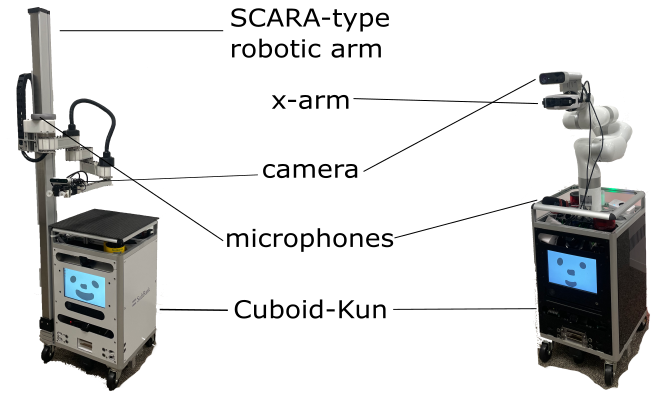
\includegraphics[width=0.5\linewidth]{images/Hardware.png}
    \caption{Image of two robots: ``MonAr'' (left) and ``Cuboid-X'' (right).}
    \label{fig:hardware}
\end{figure}

% start p.3-----------
\subsection{Mobile Base}
``Cuboid-kun'' is a self-navigating autonomous mobile robot that our team is developing. It is equipped with a computer, a power supply, and multiple sensors for obstacle avoidance. It is operated with differential drive and can carry a payload of 20~kg. The mobile base is intended to be used in houses and office buildings, and therefore has a small footprint of 370~mm inside a square. In addition, the hardware was designed to be reconfigurable, and therefore we can easily attach external modules\footnote{https://www.signagekun.com/cuboid} to the robot, such as a robotic arm.

% In-wheel motor, VESC,
% start p.4-----------
\subsection{Robotic Arm}
% SCARA arm, x-arm
``MonAr'' is equipped with a SCARA-type robotic arm designed by our team. The robot arm has 8 degrees of freedom and can carry a small payload of 500~g. The end-effector is equipped with a vacuum gripper with two suction cups and a compact RGB-D hand camera (RealSense D415). The robot arm was designed for WRS FCSC, where one of the key tasks is to rearrange multiple objects on a shelf. To handle objects within a small space, we designed the robot arm to have a large operation space with thin and compact end-effectors.

``Cuboid-X'' is equipped with xArm 7, a commercially available robot arm with 7 degrees of freedom. This robot arm is composed of large actuator modules and can carry a payload of 3.5~kg although the robot arm has small operation space compared to ``MonAr''. The end-effector is equipped with a two-finger gripper and a high-performance RGB-D hand camera (Azure Kinect).


\subsection{Microphones}
% ODAS
% Shotgun Microphone
We are currently experimenting with two different types of microphones, and plan to use the one with the better performance in the competition.
One is a highly directional microphone, which is often used in RoboCup@Home.
When the speaker is in front of the microphone, it is easier to recognize the speaker's voice. The disadvantage of using this type of microphone is that the speaker must stand in front of the microphone.

Another method we are trying is to use a microphone array module, such as XMOS, for source separation.
We use a software called ODAS~\cite{Grondin201963} to perform the source separation.
This feature enables us to recognize speech in noisy environments by separating the speaker's sound source. Furthermore, it can distinguish between two or more people speaking at the same time. Figure~\ref{fig:odas} shows the sound source localization using ODAS\_WEB.
\begin{figure}[tbp]
    \centering
    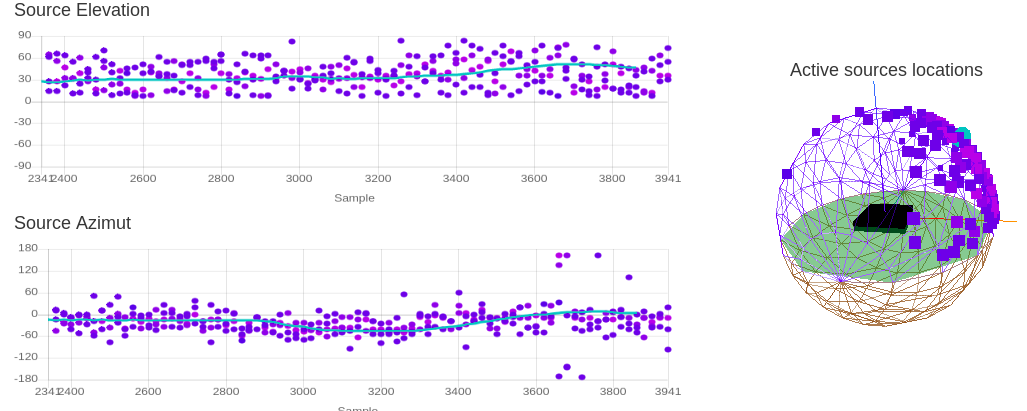
\includegraphics[width=0.6\linewidth]{images/odas_web_side.png}
    \caption{Sound source localization.}
    \label{fig:odas}
\end{figure}

\section{Software}
% Figure: System Overview
All our ``Cuboid-kun''-based robots, such as ``MonAr'' and ``Cuboid-X'', run on a common system.
The overview of our software system, shown in Fig.~\ref{fig:software}, is comprised of three main layers:
\begin{enumerate}
    \item the perception layer, collection of software modules that takes robot’s sensor data and process them to create symbolic representations of the environment,
    \item the planning layer, collection of software modules that takes the state of the environment to evaluate and generate a sequence of appropriate robot behaviors, and
    \item the control layer, collection of software modules that translates the planned behavior and sends appropriate commands to the actuators for the robot to interact with the environment.
\end{enumerate}
The primary framework for software module interaction is Robot Operating System (ROS), with each software module representing one or several ROS nodes.
\begin{figure}[tbp]
    \centering
    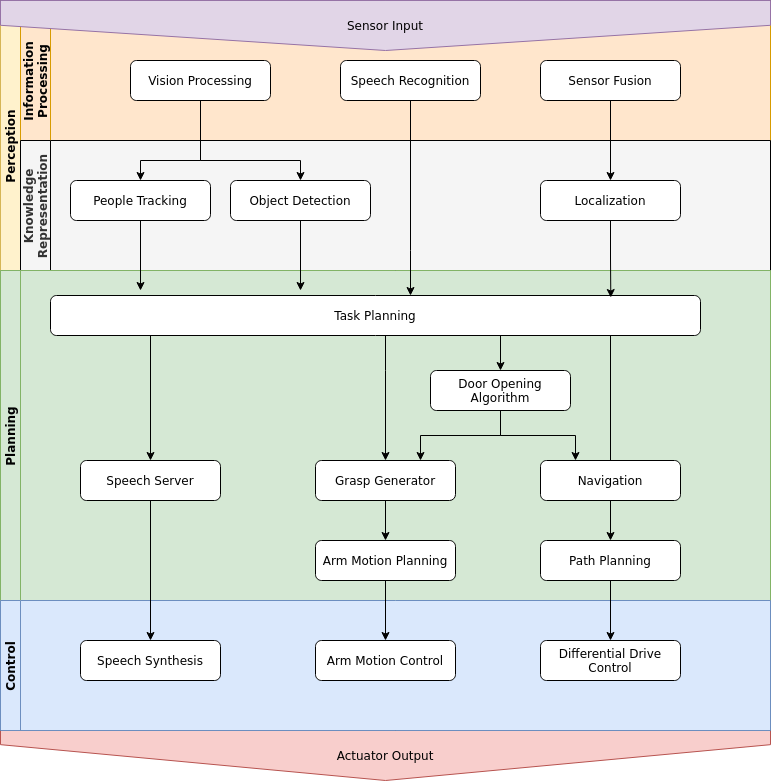
\includegraphics[width=0.6\linewidth]{images/SoftwareOverview.png}
    \caption{``Cuboid-kun'' software overview.}
    \label{fig:software}
\end{figure}


\subsection{Object Classification and Pose Estimator Algorithm}
\label{sec:pose_estimation}
% plane top object detection (jsk)
% YOLO
We mainly use ClusterPointIndices, a function of jsk\_pcl\_ros\footnote{https://github.com/jsk-ros-pkg/jsk\_recognition} ROS package, to extract the point cloud data from the object on a plane and estimate the object's pose and collision shapes.
However, for YCB objects used in RoboCup@Home league open source dataset, we used PERCH 2.0~\cite{Agarwal2020PERCH2} to estimate more accurate poses, as shown in Fig.~\ref{fig:perch}.
\begin{figure}[tbp]
    \centering
    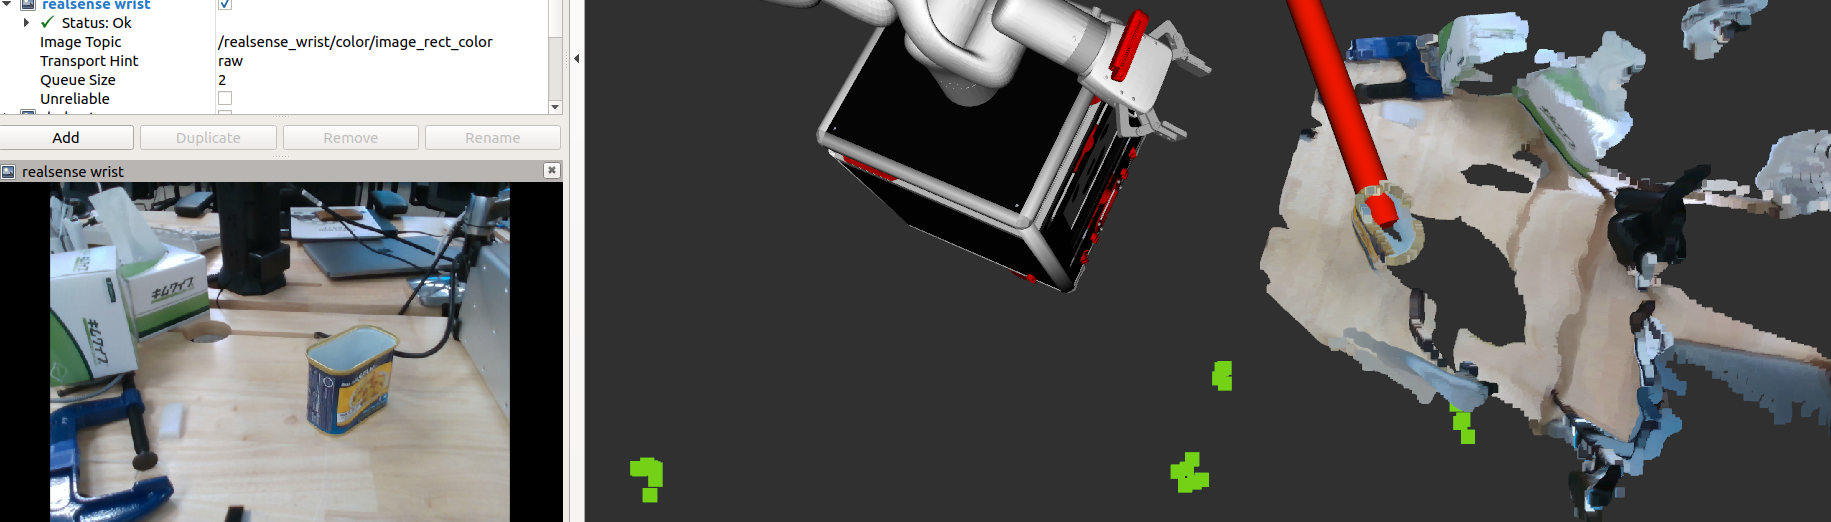
\includegraphics[width=0.6\linewidth]{images/pearch.png}
    \caption{Spam can pose estimation with PERCH 2.0.}
    \label{fig:perch}
\end{figure}

We use YOLO, trained with MSCOCO dataset, for object classification.
However, since the RoboCup@Home league requires more detailed recognition results than the MSCOCO dataset, we also use a classifier trained using GoogLeNet~\cite{Massouh2019} for unknown objects.

\subsection{Grasping Object Algorithm}
\label{sec:grasp_object}
We designed the object grasping algorithm in the following sequence. We first estimate the object poses and collision shapes using the object pose estimator algorithm as described in section~\ref{sec:pose_estimation}. We also estimate the support table’s (the area where the object resides on) collision shape and pose. After estimating the object’s pose and collision shapes along with the support table, we generate the grasp candidates using HandleEstimator, another function of jsk ROS package. Finally, we provide the calculated information to MoveIt’s\footnote{https://github.com/ros-planning/moveit} planning scene and use MoveIt’s pick and place pipeline to compute the manipulator’s trajectory path to grasp the object. Figure~\ref{fig:grasp_object} visualizes the grasping object algorithm for grasping a pet bottle.

\begin{figure}[tbp]
    \centering
    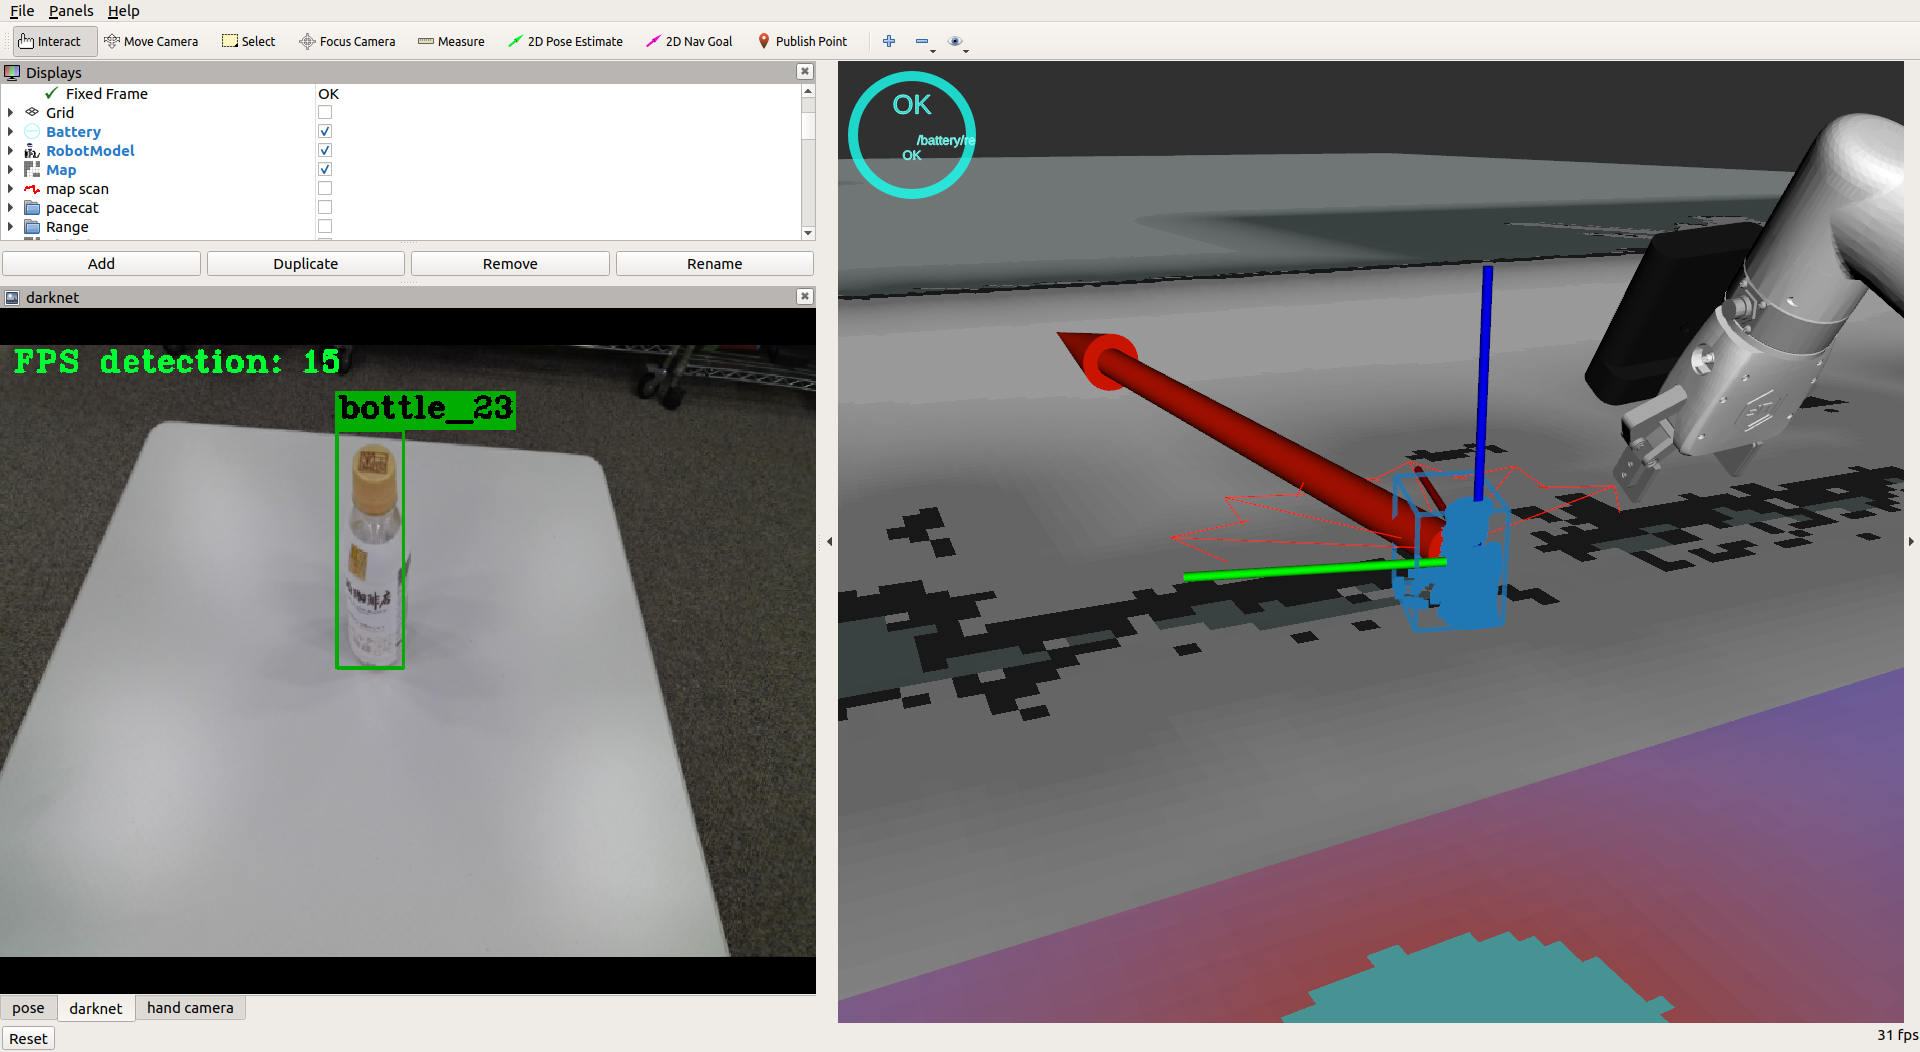
\includegraphics[width=0.6\linewidth]{images/grasp_object.png}
    \caption{Visualizing grasping object algorithm for grasping a pet bottle. The left panel shows YOLO detecting a pet bottle. The right panel shows the grasping object algorithm clustering the pet bottle’s point cloud (blue) from plane top points, estimating the pose (rgb axis), and generating the grasp poses (red arrows). The robot then selects the best grasping pose (large red arrow) to pick the pet bottle.}
    \label{fig:grasp_object}
\end{figure}

\subsection{Door Opener Algorithm}
% door detection (YOLO)
% handle pose estimation with plane estimation
% open door flow
\begin{figure}[tbp]
    \begin{tabular}{cc}
        \begin{minipage}[t]{0.45\hsize}
            \centering
            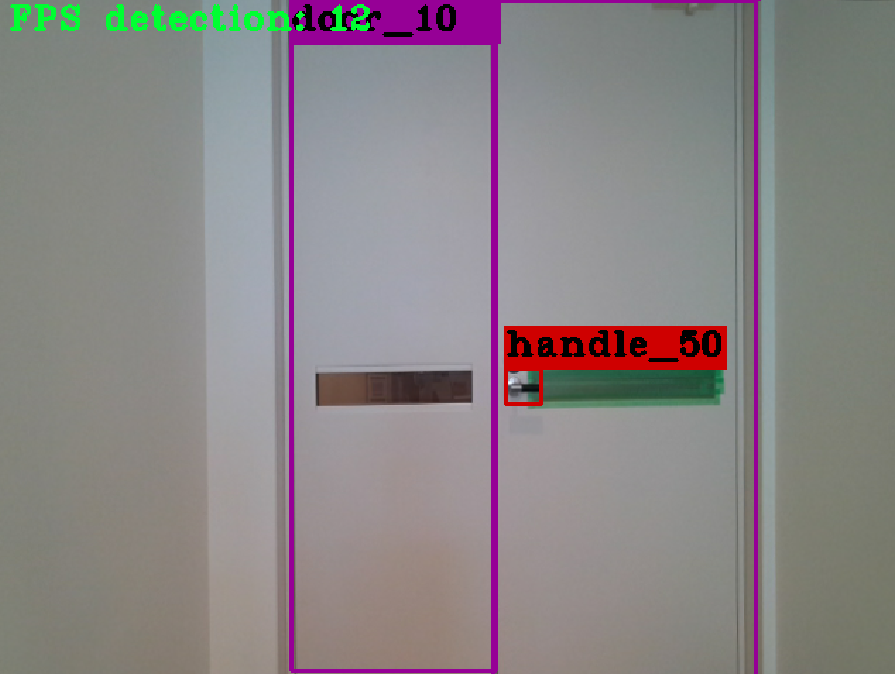
\includegraphics[width=0.8\linewidth]{images/door_yolo.png}
            \caption{Door detection with YOLO.}
            \label{fig:door_detection}
        \end{minipage}  &
        \begin{minipage}[t]{0.45\hsize}
            \centering
            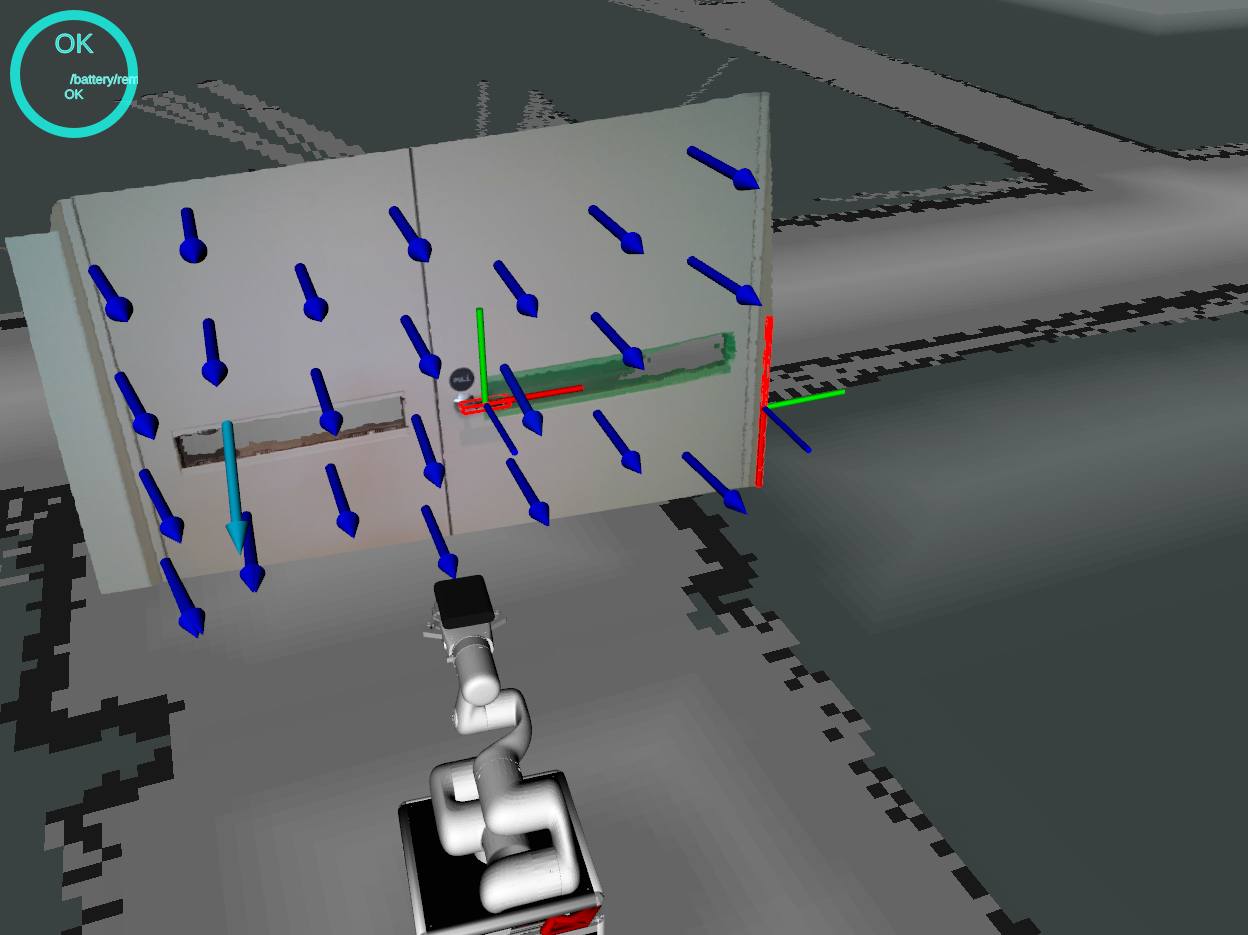
\includegraphics[width=0.8\linewidth]{images/normal.png}
            \caption{Door plane estimation.}
            \label{fig:door_plane}
        \end{minipage}    \\
        \begin{minipage}[t]{0.45\hsize}
            \centering
            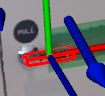
\includegraphics[width=0.4\linewidth]{images/handle_pose.png}
            \caption{Handle pose estimation.}
            \label{fig:handle_pose}
        \end{minipage} &
        \begin{minipage}[t]{0.45\hsize}
            \centering
            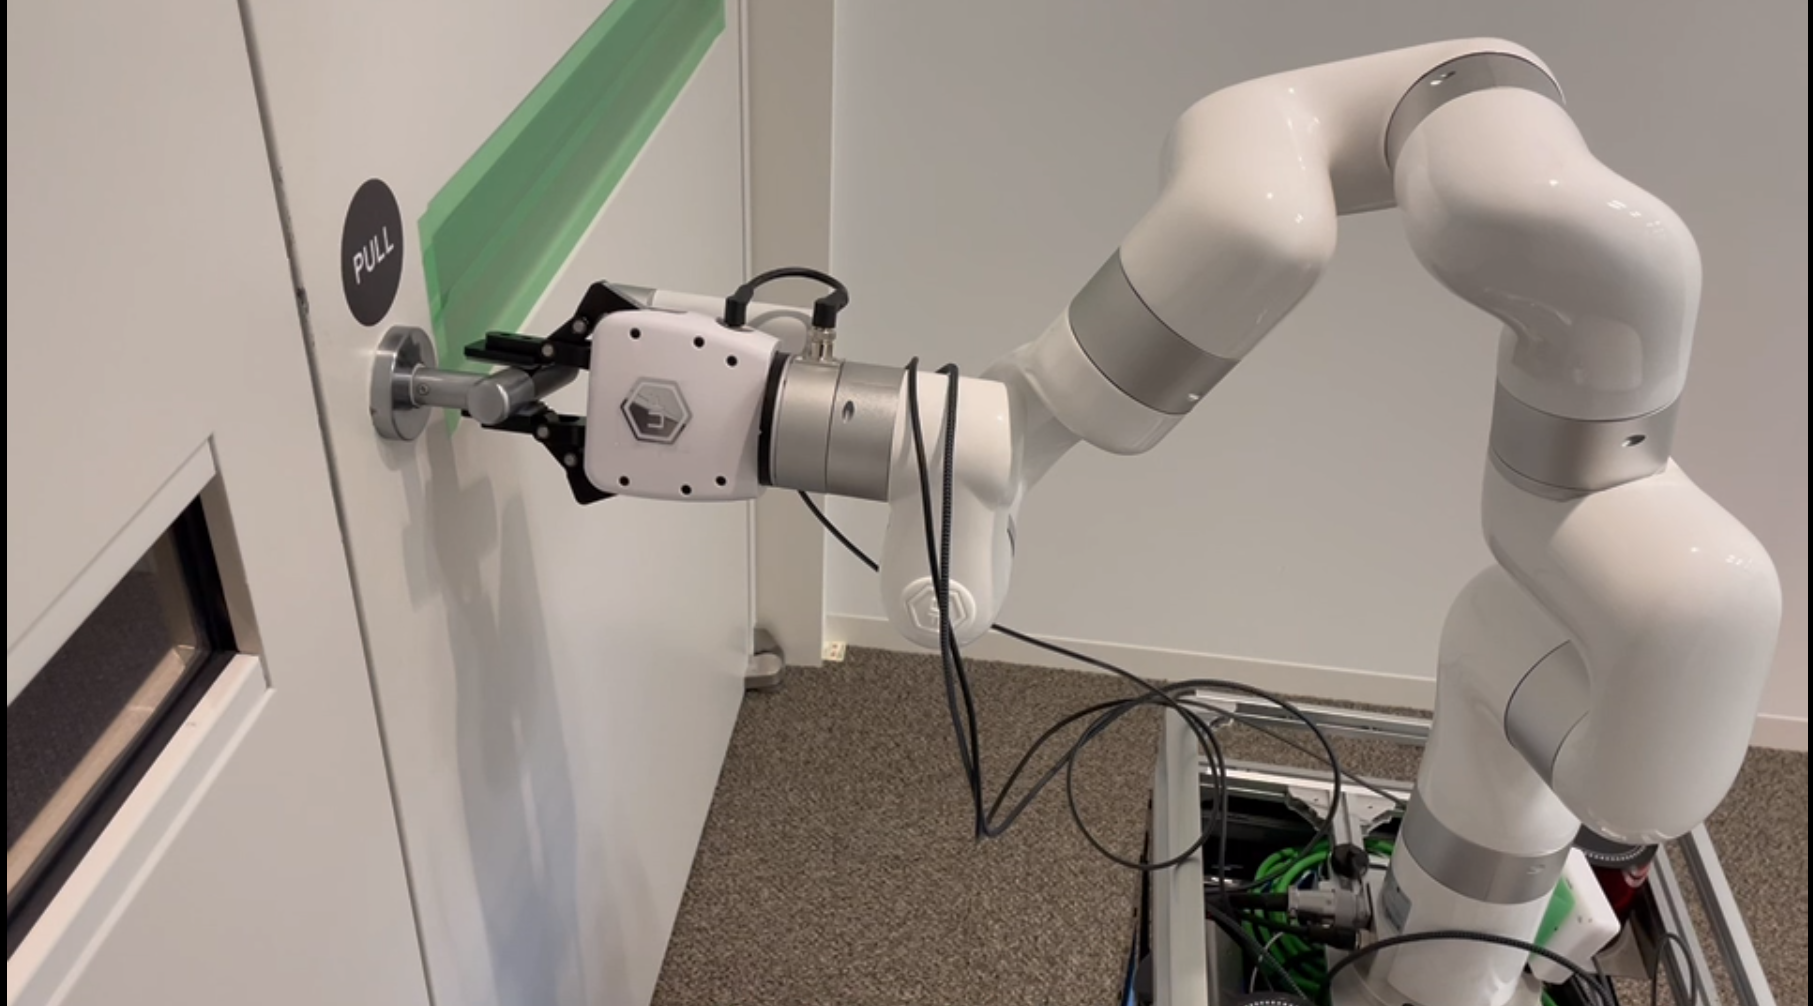
\includegraphics[width=0.8\linewidth]{images/grasp_door_handle.png}
            \caption{Result of grasping the handle.}
            \label{fig:grasp_handle}
        \end{minipage}
    \end{tabular}
\end{figure}
We designed the door opener algorithm in the following sequence. First, we use YOLO to recognize doors and handle positions.
The door dataset and the trained model of YOLO are described in \cite{Arduengo_2021}.
Figure~\ref{fig:door_detection} shows the results of door detection by YOLO.
YOLO can even detect a double-door as two doors along the center slit.
Next, we estimate the pose of the door using jsk ROS package as described in section~\ref{sec:pose_estimation}.
In Fig.~\ref{fig:door_plane}, the blue arrows represent the normal vector of the door, and in Fig.~\ref{fig:handle_pose}, the red bounding box indicates that the handle is detected on the plane of the door.
After estimating the handle pose, the robot grasps the handle using MoveIt as described in section~\ref{sec:grasp_object}.
The robot achieved door opening by moving backward in the right direction based on the position of the handle and the door.
Figure~\ref{fig:grasp_handle} shows how the robot grasped the handle based on these estimation results.

\subsection{Person Tracker Algorithm}
% spencer
% + pose, YOLO
% re-identification (deep sort)
For detecting and tracking people we use the ROS package for spencer's robot~\cite{Linder2016}.
The package can fuse several different detection results such as leg detection by 2D LiDAR and upper body detection by RGB-D.
We also developed a tracking system that is even more robust to lost targets by integrating pose estimation results by OpenPose and image recognition results by YOLO as shown in Fig.~\ref{fig:track_people}.
\begin{figure}[tbp]
    \centering
    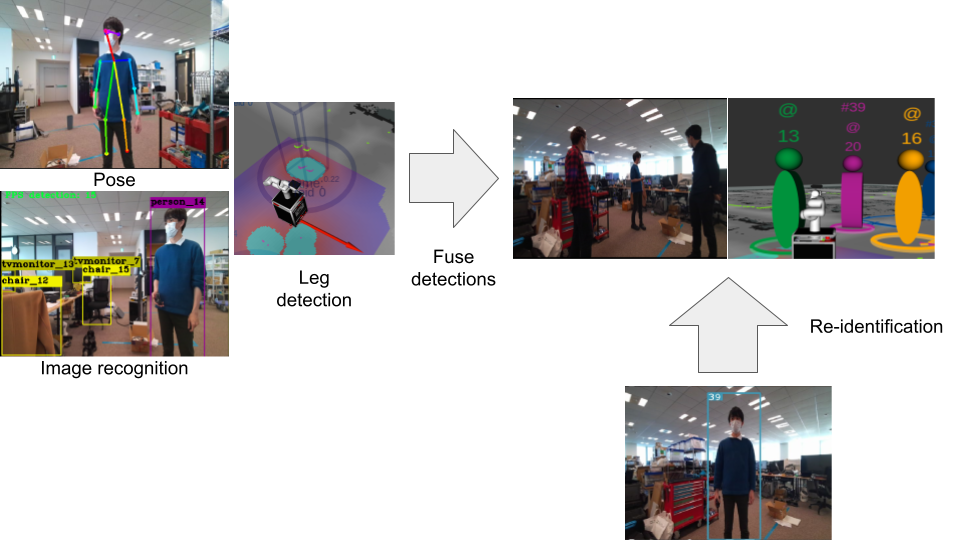
\includegraphics[width=0.8\linewidth]{images/people_track.png}
    \caption{People tracking system overview.}
    \label{fig:track_people}
\end{figure}

For pose estimation, we considered HRNet~\cite{sun2019deep} and CenterNet~\cite{zhou2019objects} as well as OpenPose.
CenterNet is a method for anchor-less object detection similar to OpenPose.
CenterNet can achieve the same processing speed with about $\frac{1}{3}$ of the GPU memory usage of OpenPose, but it assumes that all key points are always present in the bounding box.
In robotics, this result is not desirable because the whole body is often not within the angle of view of the camera.
On the other hand, HRNet provides higher performance by maintaining high resolution even during the process.
However, the processing speed is about 1~Hz, inferior to OpenPose.
HRNet is preferable to estimate poses in a static environment, but we needed to use these results in a dynamic environment for tracking, so we adopted OpenPose.

Furthermore, these tracking methods are prone to lose or swap tracking targets when the person being tracked hides in the shadows or overlaps with others.
To avoid that, we have introduced an algorithm for re-identification using Deep SORT~\cite{Wojke2018deep}.


\subsection{Speech Recognizer Algorithm}
We use the Google Speech API and Dialogflow to recognize speech phrases and responses.
We also use the snowboy\footnote{https://github.com/Kitt-AI/snowboy} to detect hotword at the start of a conversation.
Hotword triggers contribute greatly to recognizing conversational content with high accuracy, but without a sufficient number of training samples, snowboy cannot handle all of the people.
Therefore, we use hotword detection only for conversations with operators.

\section{Contribute}
As SoftBank Corp., we have sponsored various robotic competitions\footnote{https://wrs.nedo.go.jp/en/sponsor2020/}\footnote{https://tsukubachallenge.jp/2021/} and conferences\footnote{https://ac.rsj-web.org/2020/sponsorship.html}\footnote{https://roscon.ros.org/jp/2019/} to advocate human-robot interaction research. Our sister company, SoftBank Robotics Corp., is a long-term global sponsor for RoboCup. We also plan to release our software on GitHub\footnote{https://github.com/sbgisen} and share our work with other teams in the near future. Despite our low scientific contributions, we hope that our experience in RoboCup will let us develop and introduce more affordable and customizable service robots for researchers and the general population.

\section{Conclusions and future work}
In this paper, we presented how we are developing our robots for the RoboCup@Home. Using voice recognition, navigation, person tracking, and object recognition, we have implemented several tasks for RoboCup@Home. Each of these functions has its challenges in terms of speed and success rate. We will be comparing algorithms, adjusting parameters, adding functions, and debugging for the RoboCup@Home. We will also compare two different configurations of microphones and arms, and adopt the better method. What to use as a benchmark is still an issue. It is also our goal to improve the quality of the robot so that it can be commercially available.

%%%%%%%%%%%%%%%%%%%%%%%%%%%%%%%%%%%%%%%%%%%%%%%%%%%%%%%%%%%%%%%%%%%%%%%%%%%%%%%%%%%%
%
% Bibliography
%
%%%%%%%%%%%%%%%%%%%%%%%%%%%%%%%%%%%%%%%%%%%%%%%%%%%%%%%%%%%%%%%%%%%%%%%%%%%%%%%%%%%%

\bibliographystyle{unsrt}
\bibliography{bibliography}

%%%%%%%%%%%%%%%%%%%%%%%%%%%%%%%%%%%%%%%%%%%%%%%%%%%%%%%%%%%%%%%%%%%%%%%%%%%%%%%%%%%%
%
% Robot Specifications
%
%%%%%%%%%%%%%%%%%%%%%%%%%%%%%%%%%%%%%%%%%%%%%%%%%%%%%%%%%%%%%%%%%%%%%%%%%%%%%%%%%%%%

\robospecs
%CHKTEX-FILE 46

\section*{SOAR Hardware Description}%
\label{sec:annex-OPL}
% In this section briefly describe the software and hardware of the robot

\setlength\intextsep{0pt}
\begin{wrapfigure}[10]{r}{0.3\textwidth}
	\centering
	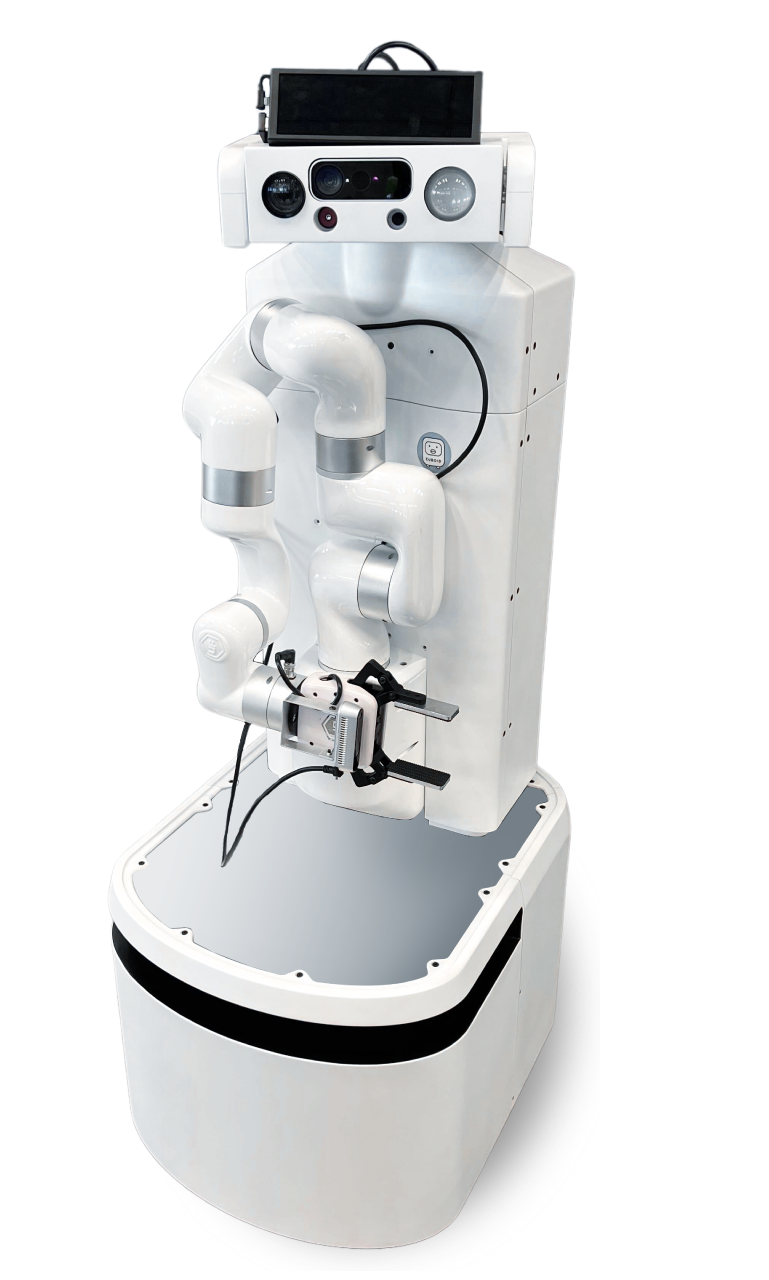
\includegraphics[width=0.4\textwidth]{images/soar.png}
	%\caption{Robot SOAR}%
	\label{fig:soar}
\end{wrapfigure}

Specifications are as follows:

\begin{itemize}
	\item Base: differential drive, 0.83 m/s max speed.
	\item Dimensions: (w) 550 mm (d) 650 mm (h) 1360 mm - 1770 mm
	\item Weight: 92 kg
	\item Arm: 8 DOF (1 DOF torso, 7 DOF manipulator)
	\item Sensors:
	      \begin{itemize}
		      \item Mobile Base:
		            \begin{itemize}
			            \item Hinson LE-50621 LiDAR
			            \item N100 9-axis IMU
		            \end{itemize}
		      \item Head:
		            \begin{itemize}
			            \item Azure Kinect RGB-D camera
			            \item ECM-SP10 microphone
			            \item JM800S-30-360X zoom camera
			            \item Seek Thermal CompactPRO Fast Frame
		            \end{itemize}
		      \item Arm:
		            \begin{itemize}
			            \item Realsense D435 RGB-D camera
		            \end{itemize}
	      \end{itemize}
	\item PC: Intel NUC (NUC11PHKi7C)
	\item Display: THANKO C-79D21B
	\item Speaker: YAMAHA VXS1MLB
\end{itemize}

\section*{SOAR Software Description}
% Please describe in this section the software you are using to control your robot. Consider the following example:

SOAR use the following software components:

\begin{itemize}
	\item Platform: Ubuntu 20.04 ROS Noetic
	\item Navigation: ROS Navigation Stack, EBand local planner
	\item Arm Motion Planner: MoveIt ROS package
	\item Object Recognition:
	      \begin{itemize}
		      \item YOLOv8
		      \item \text{jsk\_pcl\_ros} ROS package
	      \end{itemize}
	\item Behavior Architecture: SMACH ROS package
	\item Hotword: EfficientWord-Net
	\item Speech Recognition: Google Dialogflow
	\item Speech Generation: Google Text-To-Speech
	\item Person Recognition: \text{spencer\_people\_tracking} ROS package
\end{itemize}


\nocite{*}

\end{document}
